\documentclass[10pt]{beamer}

\usepackage[english]{babel}
\usepackage[utf8]{inputenc}
\usepackage{lmodern}
\usepackage{listings}
\usepackage{caption}
\usepackage{subcaption}

\captionsetup[lstlisting]{ margin=0pt }

\definecolor{lgray}{gray}{0.96}
\definecolor{lbcolor}{rgb}{0.9,0.9,0.9}
\lstset{
    framesep=2pt,
    basicstyle=\ttfamily\scriptsize,
    breaklines=true,
    breakatwhitespace=true,
    aboveskip={0.75\baselineskip},
    columns=fixed,
    showstringspaces=false,
    breaklines=true,
    frame=single,
    rulecolor=\color{lgray},
    showtabs=false,
    showspaces=false,
    showstringspaces=false,
    backgroundcolor=\color{lgray},
    identifierstyle=\ttfamily,
    keywordstyle=\color[rgb]{0,0,1},
    commentstyle=\color[rgb]{0.0,0.26,0.15},
    stringstyle=\color[rgb]{0.627,0.126,0.941}
}

\setbeamersize{text margin left=5mm,text margin right=5mm}


\usetheme{AGH}
\title{Rozbudowa i uaktualnienie systemu GGSS detektora ATLAS TRT}
\author{\normalsize{Arkadiusz Kasprzak \newline \and 
    Jarosław Cierpich \newline \newline \and 
    Opiekun pracy: dr hab. inż. Bartosz Mindur, prof. AGH}}
\date{}

\begin{document}

\renewcommand{\figurename}{Rysunek}

\titleframe[pl]

\part{Prezentacja - Arkadiusz Kasprzak}

\begin{frame}
\frametitle{Plan prezentacji - Arkadiusz Kasprzak}
\tableofcontents
\end{frame}


\section{Wprowadzenie do tematyki pracy}

\begin{frame}
\frametitle{Wprowadzenie do systemu GGSS}
\begin{itemize}
    \item System Stabilizacji Wzmocnienia Gazowego (GGSS - \emph{Gas Gain Stabilization System})
    \item projekt zintegrowany z systemem kontroli detektora ATLAS w CERN
    \item umożliwia poprawne działanie detektora TRT (\emph{Transition Radiation Tracker}) będącego częścią ATLAS
    \item składa się z warstwy oprogramowania (aplikacje oraz infrastruktura) oraz sprzętu (zasilacz wysokiego napięcia, multiplekser analogowy, wielokanałowy analizator amplitudy MCA)
    \item warstwa oprogramowania koordynuje działanie urządzeń i umożliwia sterowanie nimi za pomocą specjalnych komend
    \item aplikacje i biblioteki napisane z wykorzystaniem języka C++, infrastruktura: CMake, Bash oraz Python
\end{itemize}
% domena (CERN, TRT, DCS)
% architektura wysokopoziomowa
% warstwa sprzetowa i oprogramowania
% glowne technologie
\end{frame}

\begin{frame}
\frametitle{Wprowadzenie do systemu GGSS}
\begin{figure}
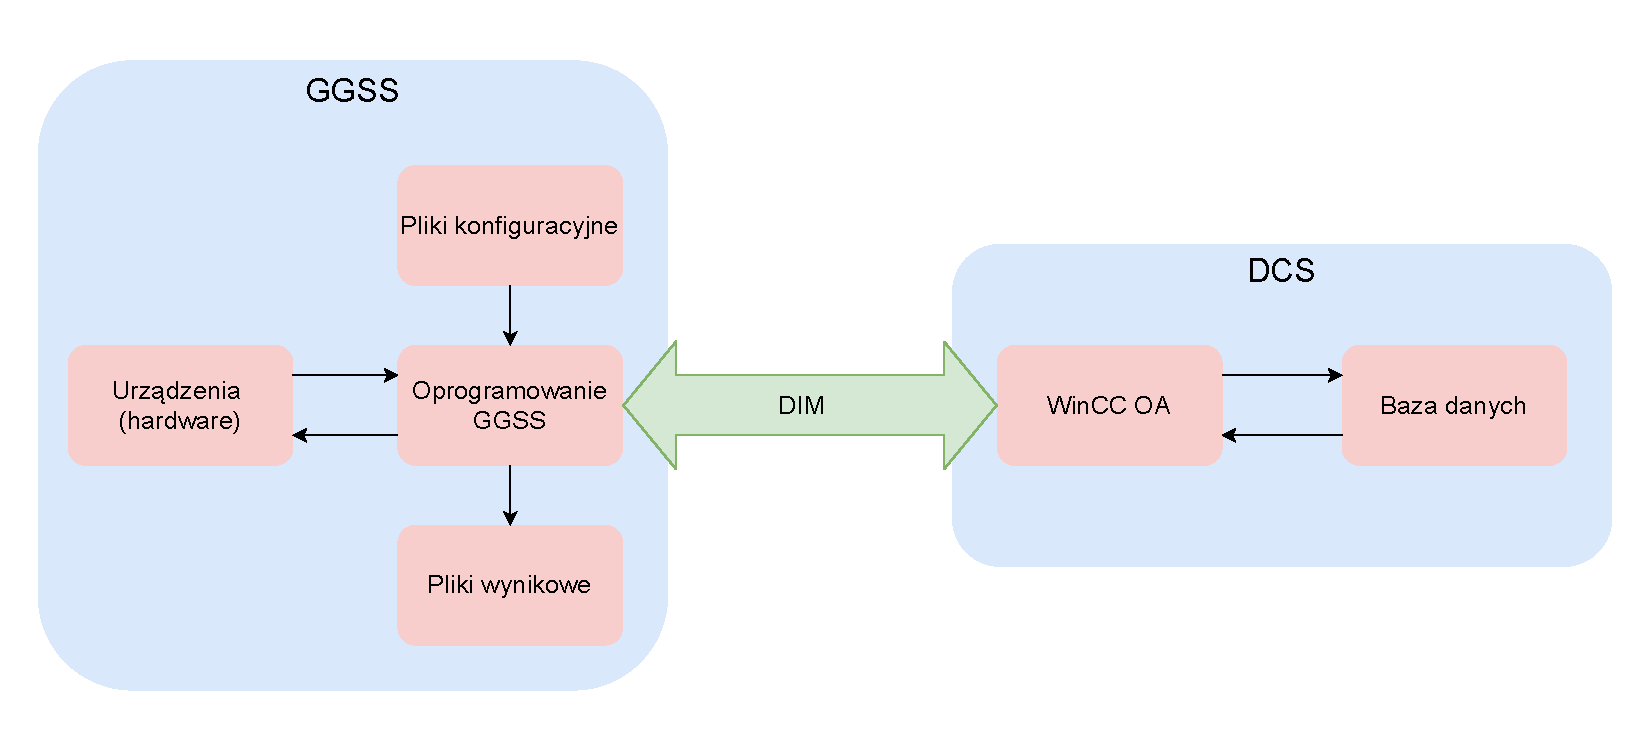
\includegraphics[width=0.85\textwidth]{static/high_level_architecture.pdf}
\caption{Wysokopoziomowa architektura systemu GGSS}
\end{figure}
\begin{itemize}
    \item WinCC OA - system system typu SCADA pozwalający na sterowanie i kontrolę działania podsystemów detektora
    \item DIM - protokół komunikacyjny dla aplikacji rozproszonych
\end{itemize}
\end{frame}

\begin{frame}
\frametitle{Cele pracy}
\begin{itemize}
    \item kontynuacja pracy inżynierskiej, skupiającej się na infrastrukturze projektu
    \item rozbudowa przygotowanych w ramach wspomnianej pracy rozwiązań
    \item główny nacisk na aplikację \emph{ggss-runner}, stanowiącą trzon systemu
    \item poprawa jakości kodu źródłowego oraz wprowadzenie nowych funkcjonalności
    \item rozbudowa infrastruktury pozwalającej na testowanie projektu
    \item udokumentowanie projektu (dokumentacja kodu źródłowego oraz pliki instruktażowe)
    \item migracja projektu - nowy komputer docelowy (początkowo planowany wyjazd do CERN, ostatecznie zrealizowana zdalnie)
    \item konieczność zachowania wysokiej niezawodności systemu - stosowanie praktyk takich jak \emph{code review} i testy automatyczne
\end{itemize}
% kontyuacja pracy inz
% zwrocic uwage na migracje i wyjazd, powiedziec ze prace zdalnie
% wymagana niezawodnosc - praktyki (code review itd)
\end{frame}

\section{Modyfikacja kodu źródłowego projektu}

\begin{frame}
\frametitle{Aplikacja \emph{ggss-runner}}
\begin{itemize}
    \item wielowątkowa aplikacja napisana z wykorzystaniem C++ i pakietu Boost
    \item zadanie: cykliczne gromadzenie danych w postaci widma poprzez komunikacje z wielokanałowym analizatorem amplitudy oraz wyznaczanie na ich podstawie wartości napięcia, komunikacja z systemem WinCC OA
\end{itemize}
\begin{figure}
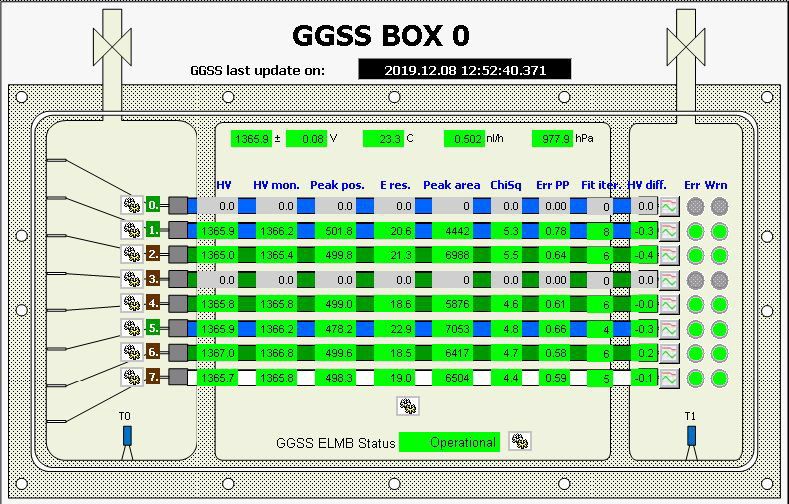
\includegraphics[width=0.6\textwidth]{static/winccoa_panel.png}
\caption{Panel dostępny w ramach systemu WinCC OA}
\end{figure}
% skrotowy opis dzialania
% wersja pierwotna - charakterystyka
\end{frame}

\begin{frame}
\frametitle{Modernizacja i poprawa jakości kodu źródłowego}
\begin{itemize}
    \item pierwotnie kod wykorzystywał standard C++03 oraz elementy C++11
    \item przeprowadzono migrację do standardu C++11 (pętle zakresowe, silne typy wyliczeniowe itd.)
    \item migracja niepełna z uwagi na ograniczenia kompilatora
    \item ujednolicono konwencje stosowane w kodzie (formatowanie, nazewnictwo)
    \item zlikwidowano niewykorzystywane lub wykomentowane fragmenty kodu
    \item usunięto nieliczne błędy (biblioteki \emph{xml-lib} oraz \emph{log-lib})
    \item znaczne zmiany w 12 z 14 bibliotek wchodzących w skład systemu
\end{itemize}
% migracja do cpp11
% poprawa błedów
\end{frame}

\begin{frame}
\frametitle{Wprowadzone funkcjonalności}
\begin{itemize}
    \item dodanie obsługi zaawansowanych komend dla zasilaczy wysokiego napięcia
    \item rozbudowa biblioteki odpowiedzialnej za dopasowanie krzywej do zebranych danych
    \item dodanie możliwości aktualizacji parametrów i zebranych danych na żądanie
    \item dodanie zabezpieczenia przed przepełnieniem bufora urządzenia MCA
    \item dodanie możliwości przywracania domyślnej kolejności liczników słomkowych
\end{itemize}
\end{frame}

\begin{frame}
\frametitle{Przykład: nowe komendy dla zasilaczy}
\begin{figure}
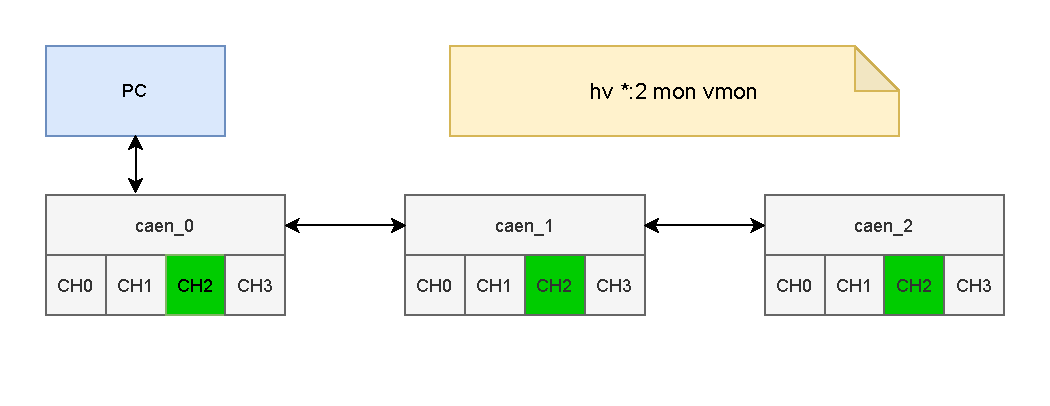
\includegraphics[width=\textwidth]{static/hv_psu_1.pdf}
\caption{Schemat przybliżający sposób działania nowego formatu komend.}
\end{figure}
\end{frame}

% TODO: moze jakis link do repo zeby pokazac 
\begin{frame}
\frametitle{Testy automatyczne}
\begin{itemize}
    \item w celu zapewnienia niezawodności i szybkiego wykrywanie błędów wykorzystano testy automatyczne i metodykę TDD (\emph{Test Driven Development})
    \item testy przygotowane z wykorzystaniem biblioteki Boost.Test
    \item uruchamiane automatycznie po wdrożeniu zmian do repozytoriów projektu
\end{itemize}
\begin{figure}
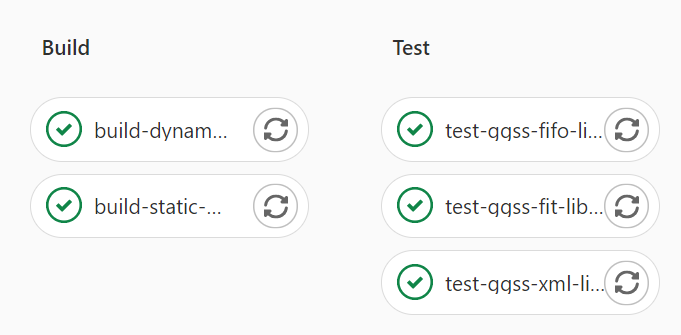
\includegraphics[width=0.65\textwidth]{static/pipeline.png}
\caption{\emph{Pipeline CI/CD} wykonujący testy automatyczne po wdrożeniu zmian}
\end{figure}
\end{frame}


\section{Modyfikacja systemu budowania projektu}

\begin{frame}[fragile]
\frametitle{Modyfikacja systemu budowania projektu}
\begin{itemize}
    \item system oparty o narzędzie CMake, przygotowany w ramach pracy inżynierskiej
    \item jego zadaniem jest obsługa projektu o hierarchicznej strukturze
    \item wsparcie dla testów automatycznych oraz generowania dokumentacji za pomocą narzędzia Doxygen
    \item system oparty o tzw. szablony - pliki \emph{.cmake} zawierające często wykorzystywane fragmenty kodu
    \item zmiana sposobu implementacji szablonów - wykorzystanie funkcji i makr
\end{itemize}
\begin{lstlisting}[caption={}]
ggss_build_static_library(
    TARGET_NAME "thread"
    DEPENDENCY_PREFIX "${CMAKE_CURRENT_SOURCE_DIR}/.."
    DEPENDENCIES "sigslot" "ggss-util-libs/log"
)
\end{lstlisting}
% cmake i czemu
% co zostalo zmienione
% wsparcie dla testow i dokumentacji
\end{frame}


\part{Prezentacja - Jarosław Cierpich}

\begin{frame}
\frametitle{Plan prezentacji - Jarosław Cierpich}
\tableofcontents
\end{frame}

\section{Modyfikacja architektury projektu}

\begin{frame}
\frametitle{Modyfikacja architektury projektu}
\framesubtitle{Poprzednia architektura projektu}
\begin{figure}
    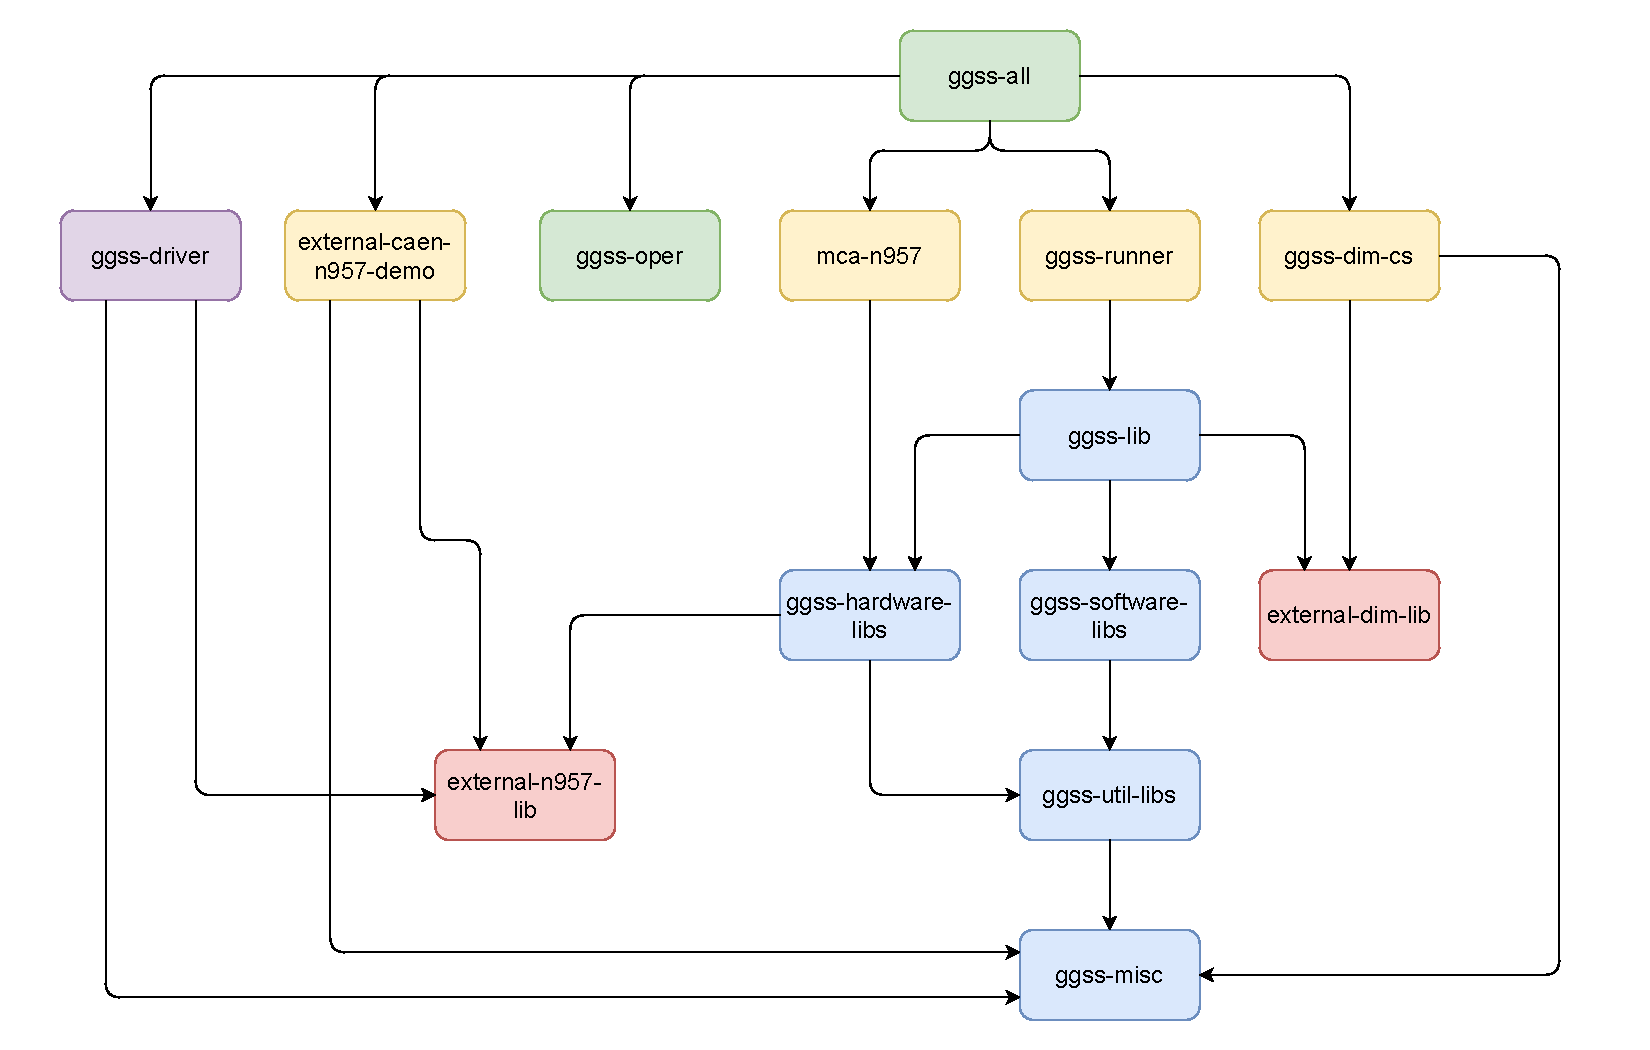
\includegraphics[width=0.8\textwidth]{static/old_structure.pdf}
    \caption{Architektura projektu na podstawie modułów oraz ich powiązań}
\end{figure}
\end{frame}

\begin{frame}
    \frametitle{Modyfikacja architektury projektu}
    \framesubtitle{Wprowadzone zmiany}
% zmiany w strukturze submodułów
% usunięcie/archiwizacja niektorzych modułów
    \begin{itemize}
        \item zmniejszenie złożoności poprzez zmniejszenie ilości modułów
        \item pozbycie się modułów, które, w trakcie prac, okazały się niepotrzebne (na~przykład: \emph{ggss-misc})
        \item wydzielenie powielonego kodu do nowej biblioteki zawartej w ramach repozytorium \emph{ggss-hardware-libs}
        \item gałęzie \emph{legacy} oraz archiwizacja projektów
    \end{itemize}
\end{frame}

\begin{frame}
\frametitle{Modyfikacja architektury projektu}
\framesubtitle{Nowa architektura projektu}
\begin{figure}
    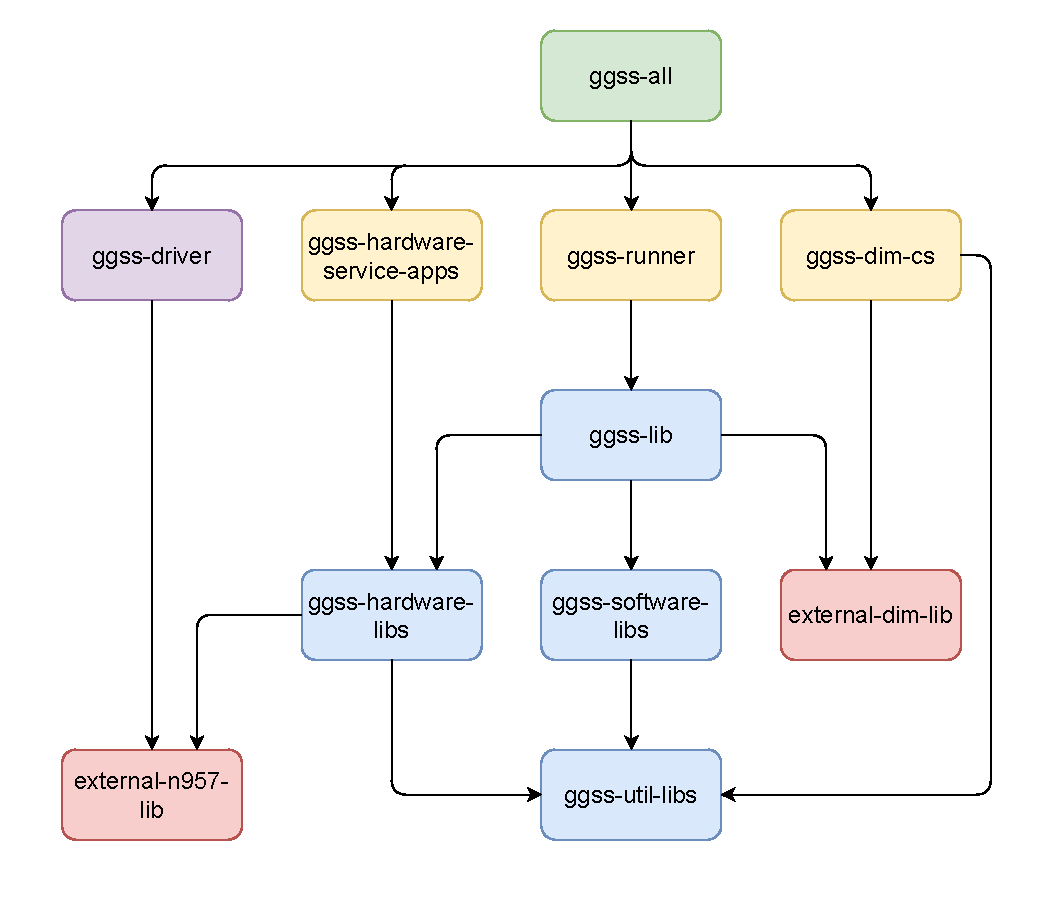
\includegraphics[width=0.6\textwidth]{static/new_architecture.pdf}
    \caption{Architektura projektu na podstawie modułów oraz ich powiązań}
\end{figure}
\end{frame}


\section{Modyfikacja infrastruktury projektu}

\begin{frame}
\frametitle{Mechanizm ciągłej integracji i dostarczania}
% co to jest
    \begin{itemize}
        \item mechanizm pozwalający na automatyczne testowanie, budowanie oraz przygotowywanie kodu do dostarczania do środowiska docelowego
        \item pierwsza wersja została utworzona w ramach pracy inżynierskiej, następnie została ona rozwinięta w ramach pracy magisterskiej
        \item do mechanizmu zostało dodane tworzenie artefaktów, a wraz z~wprowadzeniem testów automatycznych został dodany krok \emph{test}
        \item automatyzacji poddane zostało również wersjonowanie projektu
    \end{itemize}
% dodanie kroku test do wczesniejszych (build itd)
% artefakty
\end{frame}

\begin{frame}
\frametitle{Automatyzacja i centralizacja wersjonowania projektu}
    \begin{itemize}
        \item automatyzacja oparta o rozszerzenia:
            \begin{itemize}
                \item plików \emph{.cmake} w celu wsparcia parametru version
                \item skryptu \emph{build.py}, który jest nakładką narzędzia CMake
                \item mechanizmu ciągłej integracji w celu automatycznego generowania wersji na podstawie wiadomości zawartych w ramach rewizji
            \end{itemize}
        \item rozwiązanie oparte o standard \emph{semantic-versioning}, bibliotekę \emph{semantic-release} oraz konwencję oznaczania wiadomości zgodną z \emph{eslint-semantic-release}
    \end{itemize}
\begin{figure}
    
\includegraphics[width=0.7\textwidth]{static/commit}
    \caption{Rewizja zgodna z konwencją \emph{eslint-semantic-release}}
\end{figure}
% semantic-versioning i semantic-release
% zmiany w skryptach, cmake i ci/cd
\end{frame}

\begin{frame}
\frametitle{Automatyzacja pracy z submodułami}
\begin{figure}
    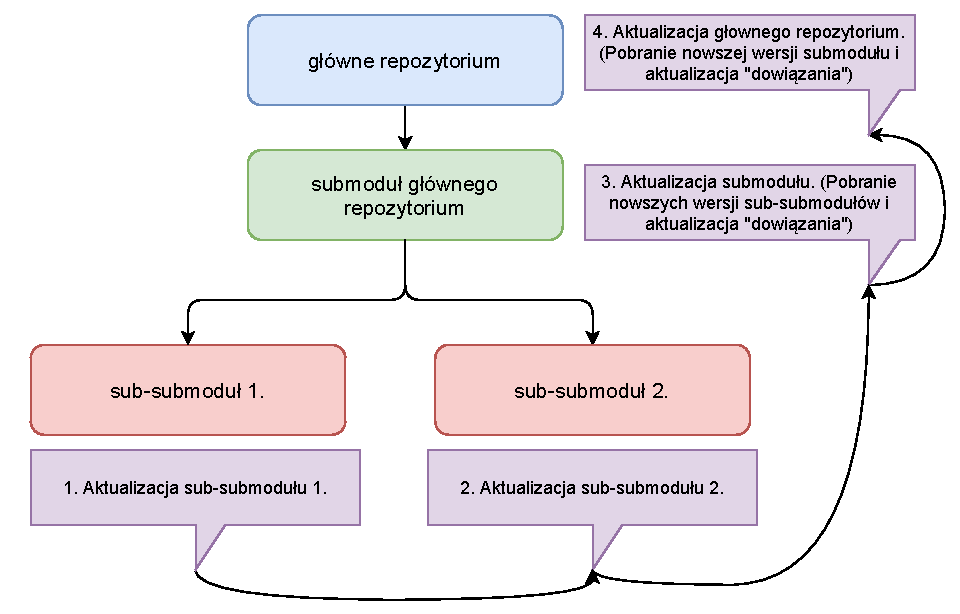
\includegraphics[width=0.75\textwidth]{static/submodules_update}
    \caption{Opis kroków jakie należy podjąć, aby wprowadzone zmiany były widoczne w całym projekcie.}
\end{figure}
% zarys problemu
\end{frame}

\begin{frame}
\frametitle{Pozostałe zmiany}
\begin{itemize}
    \item zaktualizowane zostały skrypty operacyjne, czyli skrypty obsługujące projekt GGSS w środowisku docelowym
    \item nowy skrypt monitorujący zasoby wykorzystywane przez główną aplikację projektu GGSS został utworzony
    \item przygotowana została aplikacja \emph{high-voltage-killer}, która zabezpiecza system poprzez wyłączenie zasilania na zasilaczu wysokiego napięcia
    \item dokonano modyfikacji struktury katalogów oraz nazw w środowisku docelowym
\end{itemize}
% skrypty operacyjne
% skrypt monitorujacy
% uprzatniecie maszyny docelowej
\end{frame}

\section{Aplikacje do testów urządzeń}

\begin{frame}
\frametitle{Aplikacje do testów urządzeń}
    \begin{itemize}
        \item przygotowanie aplikacji służących do testowania urządzeń - potrzeba poprawnie skonfigurowanej i działającej warstwy sprzętowej
        \item istniejące rozwiązania o ograniczonych możliwościach i niejednolitym interfejsie
        \item przygotowane rozwiązanie pozwala na dogłębne przetestowanie urządzeń z wykorzystaniem dwóch trybów: interaktywnego oraz scenariuszowego
        \item w celu dokonania odpowiednich testów wymagana jest jedynie wiedza domenowa
    \end{itemize}
% motywacja + migracja na nowy komputer i hub
% nowe rozwiazanie i jego interfejs (tryb scenariuszowy, brak koniecznosci znajomosci kodu)
% przyklad scenariusza (?)
\end{frame}

\begin{frame}
    \frametitle{Aplikacje do testów urządzeń}
    \lstinputlisting[
        caption={Przykładowy scenariusz dla zasilacza wysokiego napięcia.},
    ]{static/high-voltage-service-app-scenario.yml}
\end{frame}

\section{Testy projektu}

\begin{frame}
\frametitle{Testy projektu}
    \begin{itemize}
        \item testy nowych funkcjonalności w środowisku docelowym - po każdej znaczącej zmianie
        \item testy w trakcie i po migracji do nowego środowiska docelowego, rola autorów w migracji
        \item testy finalnej wersji projektu, testy zużycia zasobów - dedykowane skrypty oraz platforma Valgrind
    \end{itemize}
% ze byly rozne (cyklicznie i na koniec)
% testy zasobów
% wspomniec o migracji
\end{frame}

\section{Podsumowanie}

\begin{frame}
\frametitle{Podsumowanie}
\begin{itemize}
    \item przygotowany system automatyzacyjny pozwala na łatwe oraz szybkie wprowadzanie nowych zmian w projekcie
    \item wszystkie rozwiązania cechują się stosowaniem ogólnie przyjętych standardów co w połączeniu z dużym naciskiem na odpowiednią dokumentację znacząco zmniejsza próg wejścia
    \item w celu zapewnienia poprawnego działania wszystkie zmiany zostały przetestowane w środowisku docelowym
    \item stosowanie nowoczesnych praktyk takich jak testy automatyczne pozytywnie wpłynęło na proces rozwoju oprogramowania
\end{itemize}
\end{frame}


\end{document}